\documentclass{article}
\usepackage[utf8]{inputenc}
\usepackage[english, spanish]{babel}
\usepackage[dvips]{graphics}
\usepackage{amsmath}
\usepackage{amssymb}
\usepackage{fullpage}
\usepackage{epsfig}
\usepackage{multicol}
\usepackage{wasysym}

\usepackage[usenames,dvipsnames]{xcolor} 
\usepackage{hyperref} 
\definecolor{linkcolour}{rgb}{0,0.2,0.6} 
\hypersetup{colorlinks,breaklinks,urlcolor=linkcolour,linkcolor=linkcolour} 

\parindent 0pt
\parskip 0pt

\newcommand{\bbZ}{\mathbb{Z}}


\begin{document}


\includegraphics[width=2cm]{uc.png}
\vspace*{-1.9cm}

\hspace*{2.1cm}
 \begin{tabular}{l}
  \sc Pontificia Universidad Católica de Chile \\
  \sc Escuela de Ingeniería \\
  \sc Departamento de Ciencia de la Computación
  %\vspace{15\baselineskip}\mbox{}
  %\vspace{-3mm}\mbox{}
 \end{tabular}
 \bigskip

\vspace*{5mm}
\begin{center}
{IIC2413 --- Bases de Datos --- 2' 2019} \\
\vspace{3mm}
{\Large\bf Entrega 2} \\
\vspace{2mm}
Matías Reyes \\
Nicolás Van Sint Jan
\end{center}

\section{Diagrama E/R}

\begin{figure}[h]	
	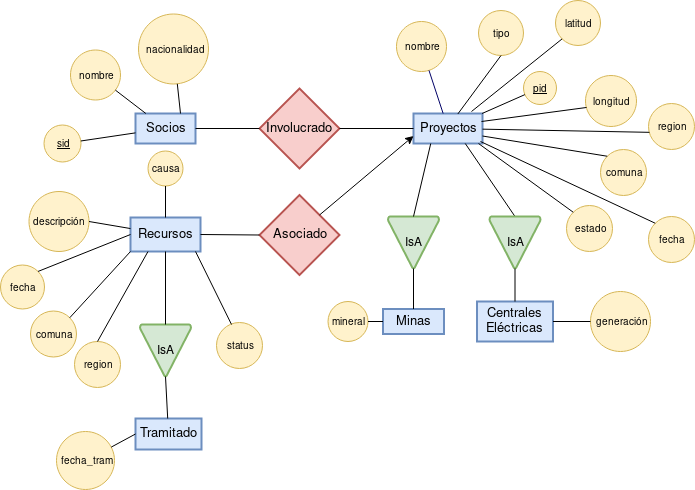
\includegraphics[width=\textwidth]{ER_v1.png}
	\caption{Diagrama Entidad/Relación}
\end{figure}

\pagebreak

\section{Esquema}
Notación
	\begin{itemize}
		\item \underline{subrrayado}: Llave primaria
		\item \textit{cursiva}: Llave foránea
	\end{itemize}
Esquema

	\begin{itemize}
		\item \texttt{Socios(\underline{snombre}: string, \underline{apellido}: string, nacionalidad: string)} 
		\item \texttt{Proyectos(\underline{pnombre}: string, latitud: float, longitud: float, \textit{comuna}: string,\\ fecha\_apertura: string, operativo: boolean, tipo: string)} 
		\item \texttt{Recursos(\underline{numero}: string, causa: string, area: float, descripcion: string,\\ fecha\_apertura: string, \textit{comuna}: string, status: string)}
		\item \texttt{RecursosProyectos(\underline{\textit{numero}}: string, \textit{pnombre}: string)} 
		
		\item \texttt{SociosProyectos(\textit{snombre}: string, \textit{apellido}: string, \textit{pnombre}: string)} 
		 
		\item \texttt{Mineras(\underline{\textit{pnombre}}: string, mineral: string)} 
		\item \texttt{Centrales(\underline{\textit{pnombre}}: str, generacion: string)} 
		\item \texttt{Tramitados(\underline{\textit{numero}}: string, fecha\_dictamen: string)} 
		
		\item \texttt{Comunas(\underline{comuna}: string, region: string)} 
	\end{itemize}

\subsection{BCNF}
	El esquema anterior está casi en 3NF porque los atributos que no son llave en cada tabla no dependen de un atributo que no sea llave, con la única excepción del atributo \texttt{comuna} que depende de la \texttt{latitud} y \texttt{longitud} (\texttt{latitud,longitud} $\rightarrow$ \texttt{comuna}) y \texttt{latitud,comuna} no es llave candidata en \texttt{Proyectos}. No consideramos este caso por ser de precisión geográfica exacta, hacer una tabla que rompa la dependencia sería redundante y consumiría espacio de más (tener un proyecto localizado en el mismo lugar que otro proyecto no tiene mucho sentido). Aún así, para poder obtener de manera correcta 3NF debemos crear una nueva relación \texttt{Localizacion(\underline{latitud}: string, \underline{longitud}:string, comuna:string)} y redifinir \texttt{Proyectos} quitando el atributo \texttt{comuna}.\\

	Con el cambio anterior, el esquema además está en BCNF dado que está en 3NF y no hay dependencias que no sean superconjuntos de llaves candidatas. Esto primero se da porque todas las relaciones tienen o una llave candidata o ninguna con la excepción de \texttt{Socios}; como ya vimos que están en 3NF, todas los atributos dependen de alguna  llave, luego es trivial que se cumpla que son superconjuntos de las llave candidata (pues tienen a lo más un elemento). El único caso especial es en la relación \texttt{Socios}, pero en este caso la dependencia es que \texttt{snombre,apellido} $\rightarrow$ \texttt{nacionalidad}, es decir, es superconjunto de la llave candidata. 

\section{Comandos usados para crear tablas}

\begin{verbatim}
DROP TABLE IF EXISTS Socios;
CREATE TABLE Socios(
	snombre VARCHAR(100),
	apellido VARCHAR(100),
	nacionalidad VARCHAR(100));
\COPY Socios FROM 'psql_socios.csv' DELIMITERS ',' CSV HEADER;


DROP TABLE IF EXISTS Proyectos;
CREATE TABLE Proyectos(
	tipo VARCHAR(20),
	pnombre VARCHAR(100) PRIMARY KEY, 
	latitud FLOAT, 
	longitud FLOAT, 
	comuna VARCHAR(50), 
	fecha_apertura DATE, 
	operativo BOOLEAN);
\COPY Proyectos FROM 'psql_proyectos.csv' DELIMITERS ',' CSV HEADER;


DROP TABLE IF EXISTS Recursos;
CREATE TABLE Recursos(
	numero CHAR(14) PRIMARY KEY, 
	causa VARCHAR(100), 
	area FLOAT, 
	descripcion TEXT, 
	fecha_apertura DATE, 
	comuna VARCHAR(50), 
	status VARCHAR(20));
\COPY Recursos FROM 'psql_recursos.csv' DELIMITERS ',' CSV HEADER;

DROP TABLE IF EXISTS Mineras;
CREATE TABLE Mineras(
	mineral VARCHAR(50), 
	pnombre VARCHAR(100) PRIMARY KEY, 
	FOREIGN KEY (pnombre) REFERENCES Proyectos (pnombre) ON DELETE CASCADE);
\COPY Mineras FROM 'psql_mineras.csv' DELIMITERS ',' CSV HEADER;

DROP TABLE IF EXISTS Comunas;
CREATE TABLE Comunas(
	comuna VARCHAR(50) PRIMARY KEY, 
	region VARCHAR(100));
\COPY Comunas FROM 'psql_comunas.csv' DELIMITERS ',' CSV HEADER;

DROP TABLE IF EXISTS Centrales;
CREATE TABLE Centrales(
	pnombre VARCHAR(100) PRIMARY KEY, 
	generacion VARCHAR(50),  
	FOREIGN KEY (pnombre) REFERENCES Proyectos (pnombre) ON DELETE CASCADE);
\COPY Centrales FROM 'psql_centrales.csv' DELIMITERS ',' CSV HEADER;

DROP TABLE IF EXISTS Tramitados;
CREATE TABLE Tramitados(
	fecha_dictamen DATE, 
	numero CHAR(14) PRIMARY KEY, 
	FOREIGN KEY (numero) REFERENCES Recursos (numero) ON DELETE CASCADE);
\COPY Tramitados FROM 'psql_tramitados.csv' DELIMITERS ',' CSV HEADER;

DROP TABLE IF EXISTS SociosProyectos;
CREATE TABLE SociosProyectos(
	apellido VARCHAR(100), 
	pnombre VARCHAR(100), 
	snombre VARCHAR(100), 
	FOREIGN KEY (apellido, snombre) REFERENCES Socios (apellido, snombre) ON DELETE CASCADE,
	FOREIGN KEY (pnombre) REFERENCES Proyectos (pnombre) ON DELETE CASCADE);
\COPY SociosProyectos FROM 'psql_syp.csv' DELIMITERS ',' CSV HEADER;

DROP TABLE IF EXISTS RecursosProyectos;
CREATE TABLE RecursosProyectos(
	numero CHAR(14) PRIMARY KEY,
	pnombre VARCHAR(100), 
	FOREIGN KEY (pnombre) REFERENCES Proyectos (pnombre) ON DELETE CASCADE,
	FOREIGN KEY (numero) REFERENCES Recursos (numero) ON DELETE CASCADE);
\COPY RecursosProyectos FROM 'psql_ryp.csv' DELIMITERS ',' CSV HEADER;
\end{verbatim}


\section{Consultas}

\begin{enumerate}
	\item \begin{verbatim}
SELECT pnombre FROM Centrales
WHERE generacion='termoeléctrica';
\end{verbatim}

\item \begin{verbatim}
SELECT pnombre FROM Proyectos NATURAL JOIN Comunas 
WHERE tipo='vertedero'
AND region LIKE '%Metropolitana%';
\end{verbatim}

\item \begin{verbatim}
SELECT numero FROM 
Recursos NATURAL JOIN RecursosProyectos NATURAL JOIN Mineras
WHERE fecha_apertura >= '1990-01-01' AND fecha_apertura <= '2010-12-31';
\end{verbatim}

\item \begin{verbatim}
SELECT DISTINCT region FROM
Recursos NATURAL JOIN Comunas
WHERE status='en trámite';
\end{verbatim}

\item \begin{verbatim}
SELECT apellido, snombre, pnombre, count FROM
(SELECT pnombre, COUNT(*) AS count FROM
Recursos NATURAL JOIN RecursosProyectos
WHERE status='en trámite'
GROUP BY pnombre) AS np NATURAL JOIN SociosProyectos 
ORDER BY 
apellido,
count DESC;
\end{verbatim}

\item \begin{verbatim}
SELECT DISTINCT Proyectos.pnombre FROM Recursos, RecursosProyectos, Proyectos 
WHERE Proyectos.pnombre=RecursosProyectos.pnombre 
AND Recursos.numero=RecursosProyectos.numero
AND Recursos.status='aprobado'
AND Proyectos.operativo=TRUE;
\end{verbatim}

\end{enumerate}

\section{Supuestos extra}
\begin{itemize}
	\item Dado que existían mineras con múltiples minerales, se decidió dejar solo uno (el primero de la lista en los datos originales) para poder usar la llave primaria del nombre de la minera (como se sugiere en la issue \href{https://github.com/IIC2413/Syllabus-2019-2/issues/50}{\#50}).
\end{itemize}


\end{document}


